\clearpage
\thispagestyle{empty}
\null
\newpage

\cleardoublepage
\phantomsection
\markboth{\spacedlowsmallcaps{Annexes}}{\spacedlowsmallcaps{Annexes}}
\part*{Annexes}
\label{part:annexes}

\clearpage
\thispagestyle{empty}
\null
\newpage

\chapter{Notations de la méthode MAMAD}\label{appendix:notations}

\section{Notations générales}

\begin{itemize}
       \item $S$ : ensemble des états possibles.
       \item $A_i$, $A$ : ensemble des actions de l'agent $i$, et ensemble conjoint des actions.
       \item $\Omega_i$, $\Omega$ : espace des observations de l'agent $i$, et espace conjoint.
       \item $H$, $H^{joint}$ : ensemble des historiques individuels et conjoints.
       \item $T$, $T_j$ : fonction de transition de l'environnement ou du jumeau numérique.
       \item $R$, $R^E_t$, $R^G_t$, $R^j_H$ : fonction de récompense (générale, par environnement, par objectif, ou basée sur les historiques).
       \item $\gamma \in [0,1]$ : facteur d'actualisation.
       \item $\pi_i$, $\pi$, $\pi^{joint}$ : politique individuelle, politique globale, politique conjointe.
       \item $\pi^*$ : politique optimale.
       \item $V^\pi$, $V^{\pi^j}_{T_j}$ : fonction de valeur ou fonction observation-valeur adaptée.
       \item $d \in D$ : un Dec-POMDP défini comme $d = (S,\{A_i\},T,R,\{\Omega_i\},O,\gamma)$.
       \item $d \in OD$ : un Observation-based Dec-POMDP (ODec-POMDP) défini comme $d = (\Omega, A, \mathcal{T}^j, \Omega^{\mathcal{T}^j}_0, R^j_H, S^j_H, \texttt{Render}^j_H, \gamma)$.
       \item $\tilde{h}_t$ : état caché récurrent estimé par le World Model.
\end{itemize}

\section{Notations pour l'activité de modélisation (MOD)}

\begin{itemize}
       \item $G_{\text{inf}}$ : objectif global informel.
       \item $S_{\text{inf}}$ : contraintes organisationnelles informelles.
       \item $E$ : description de l'environnement réel.
       \item $\Omega^j_0$ : ensemble des observations initiales conjointes.
       \item $(Enc, Dec)$ : auto-encodeur utilisé pour compresser et reconstruire les observations.
       \item $z_t$ : représentation latente d'une observation.
       \item $T_z$ : modèle récurrent de dynamique latente (RLDM).
       \item $T_j(h,\omega,a) = \langle \tilde{h}', P(\omega'|h,\omega,a)\rangle$ : JOPM prédisant la prochaine observation et mettant à jour l'état caché.
       \item $S^j_H$ : fonction d'arrêt basée sur les historiques.
       \item $Render^j_H$ : fonction optionnelle de rendu de trajectoires.
       \item $DH_j$ : ensemble d'historiques conjoints utilisés pour l'entraînement.
\end{itemize}

\section{Notations pour l'activité d'entraînement (TRN)}

\begin{itemize}
       \item $MM = \langle OS, ar, rcg, gcg, rag, rrg, grg \rangle$ : spécification MOISE+MARL.
       \item $ar : A \to R$ : relation assignant les agents à des rôles.
       \item $rcg : R \to \{rag, rrg\}$ : relation associant un rôle à un guide de contrainte.
       \item $gcg : G \to grg$ : relation liant un objectif à une contrainte.
       \item $rag(h,\omega)$ : guide d'actions attendu.
       \item $rrg(h,\omega,a)$ : guide de récompenses de rôle.
       \item $grg(h)$ : guide de récompenses d'objectifs.
       \item $\rho_i$ : rôle assigné à l'agent $i$.
       \item $m \in M$, $G_m$ : mission $m$ et ses objectifs associés.
       \item $cht$ : probabilité de conformité stricte à un rôle.
       \item $B$ : buffer d'expérience (transitions encodées).
\end{itemize}

\section{Notations pour l'activité d'analyse (ANL)}

\begin{itemize}
       \item $OF$ : Organizational Fit (adéquation organisationnelle globale).
       \item $SOF$, $FOF$ : Structural et Functional Organizational Fit.
       \item $D_{trans}$ : ensemble de séquences de transitions $(\omega_t, a_t, \omega_{t+1})$.
       \item $D_{obs}$ : ensemble de séquences d'observations $(\omega_t)$.
       \item $p \in P$ : Trajectory-based Pattern.
       \item $sl = \langle h, \{c_{min},c_{max}\}\rangle$ : séquence feuille (historique-cardinalité).
       \item $sn = \langle \langle sl_1, sl_2, ...\rangle, \{c_{min},c_{max}\}\rangle$ : séquence nœud.
       \item $l \in L$ : étiquette assignée à une observation ou action.
       \item $bg : H \to \{0,1\}$ : fonction testant l'appartenance d'un historique à un ensemble $H_g$.
\end{itemize}

\section{Notations pour l'activité de transfert (TRF)}

\begin{itemize}
       \item $\pi^{\text{latest}}_j$ : politique conjointe la plus récente.
       \item $need\_update$ : signal indiquant la nécessité d'une mise à jour.
       \item $launch\_update()$ : procédure déclenchant la mise à jour du modèle/politique.
       \item $batch\_size$ : taille minimale de $B$ pour déclencher une mise à jour.
       \item Modes de déploiement : DIRECT (local), REMOTE (distant).
\end{itemize}

\clearpage
\thispagestyle{empty}
\null
\newpage

\chapter{Détails supplémentaires sur CybMASDE}

\section{Interface graphique de CybMASDE}\label{appendix:cybmasde-gui}

\acn{CybMASDE} propose une interface graphique web développée avec le framework Angular, permettant de configurer, exécuter et analyser des projets de manière interactive. Cette interface offre une alternative à l'utilisation en ligne de commande (CLI), tout en conservant la possibilité d'automatiser les processus via des scripts. Les figures \autoref{fig:cybmasde_screenshot_configuration}, \autoref{fig:cybmasde_screenshot_training}, \autoref{fig:cybmasde_screenshot_analyzing}, et \autoref{fig:cybmasde_refining_screenshot} illustrent respectivement les onglets dédiés à la configuration du projet, à l'entraînement des politiques, à l'analyse des politiques entraînées, et au raffinement et transfert des politiques.

\begin{figure}[h!]
       \centering
       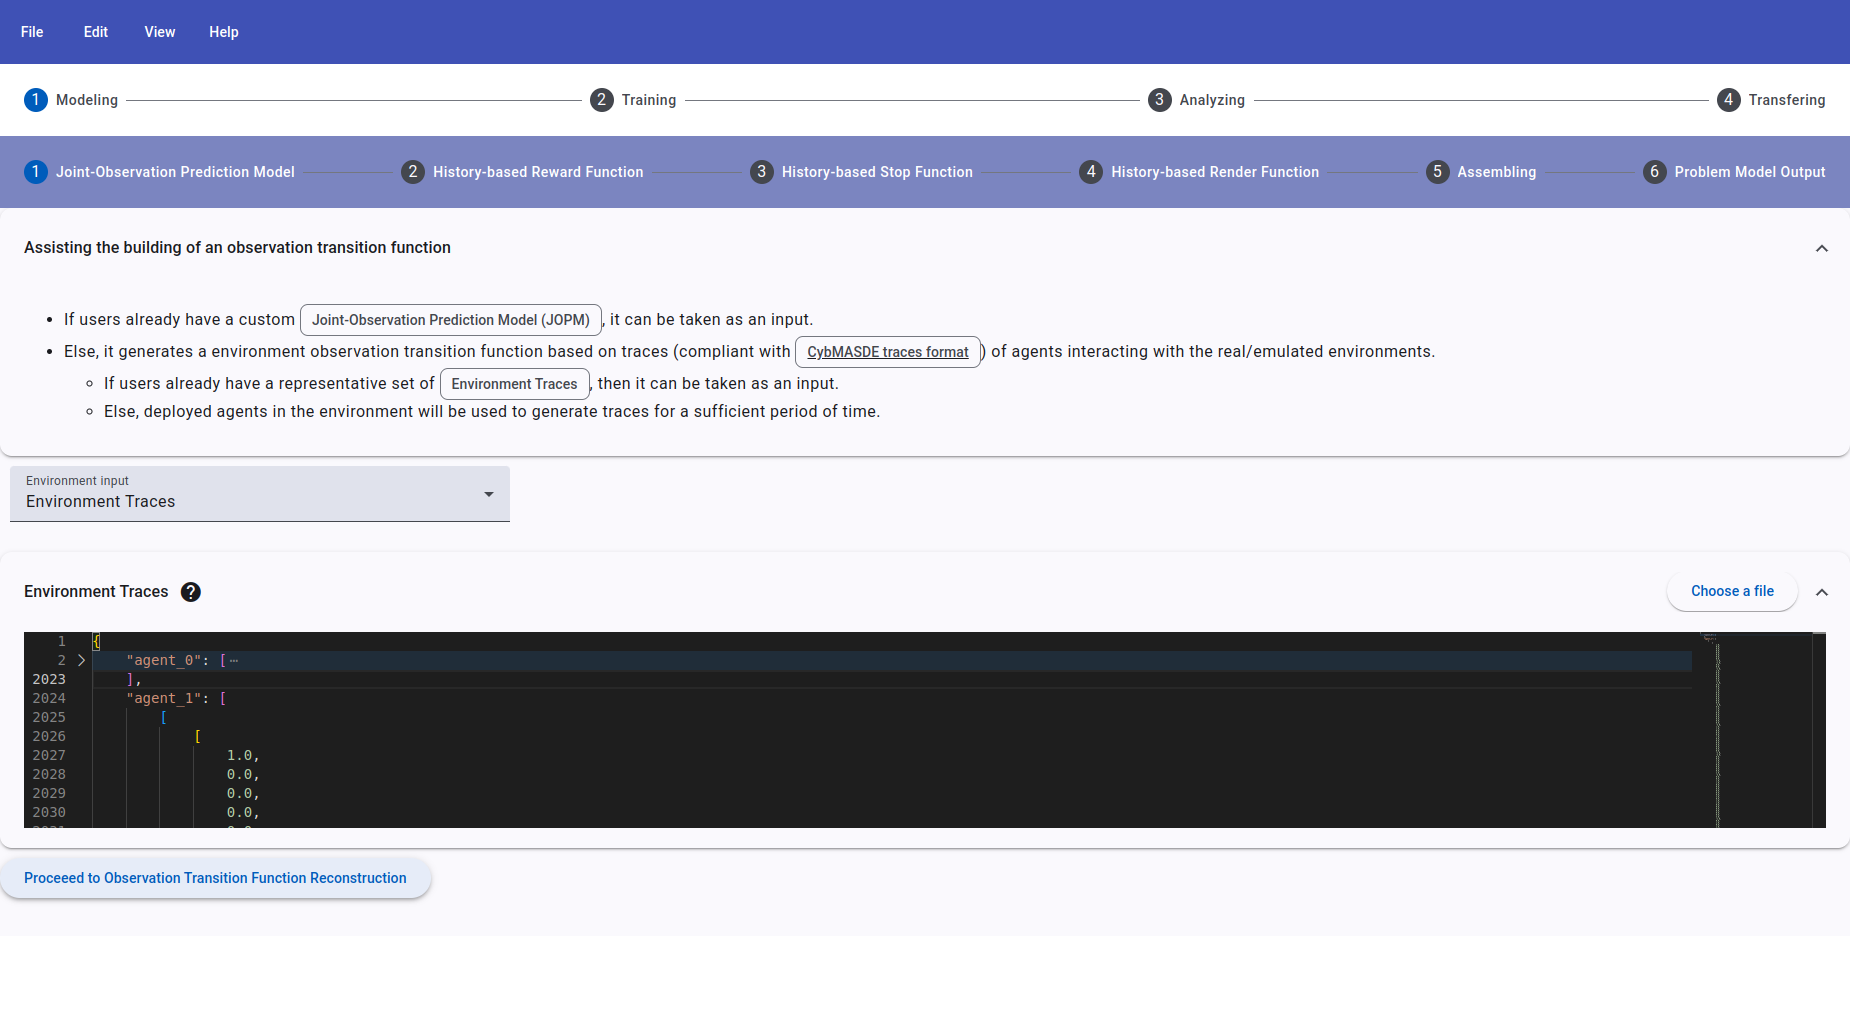
\includegraphics[width=\linewidth]{figures/CybMASDE_2.png}
       \caption[Capture d'écran de l'onglet modélisation de l'interface graphique de CybMASDE]{Capture d'écran de l'interface graphique d'édition du fichier de configuration du projet CybMASDE, illustrant ici l'onglet dédié à la modélisation. Dans cet onglet, l'utilisateur peut configurer les paramètres liés à la modélisation de l'environnement, tels que le choix entre un environnement fait main (handcrafted) ou basé sur un World Model, ainsi que les hyperparamètres associés aux modèles d'apprentissage profond utilisés pour la modélisation.}
       \label{fig:cybmasde_screenshot_configuration}
\end{figure}

\begin{figure}[h!]
       \centering
       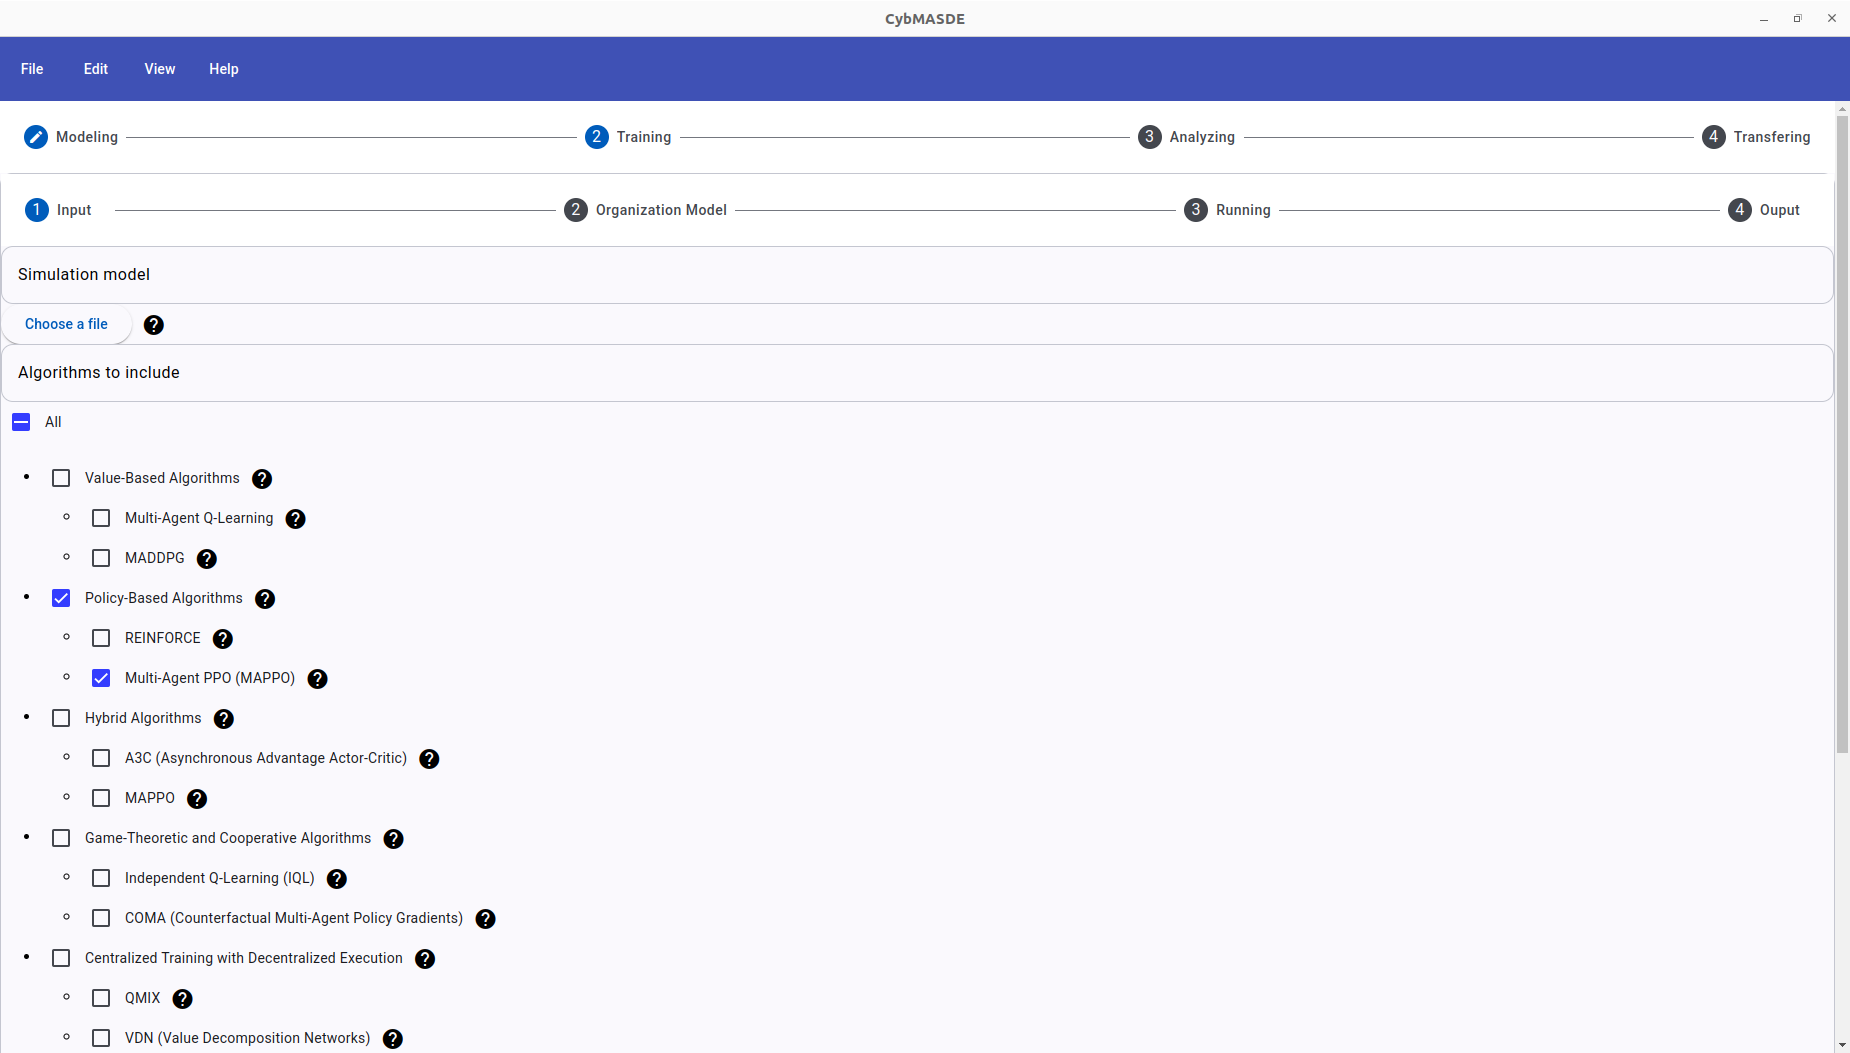
\includegraphics[width=\linewidth]{figures/training_screenshot.png}
       \caption[Capture d'écran de l'onglet entraînement de l'interface graphique de CybMASDE]{Capture d'écran de l'interface graphique d'édition du fichier de configuration du projet CybMASDE, illustrant ici l'onglet dédié à l'entraînement. Dans cet onglet, l'utilisateur peut configurer les paramètres liés à l'entraînement des politiques multi-agents, tels que le choix de l'algorithme MARL, les hyperparamètres d'entraînement (taille de batch, taux d'apprentissage, facteur de discount, etc.), ainsi que les spécifications organisationnelles MOISE+MARL.}
       \label{fig:cybmasde_screenshot_training}
\end{figure}

\begin{figure}[h!]
       \centering
       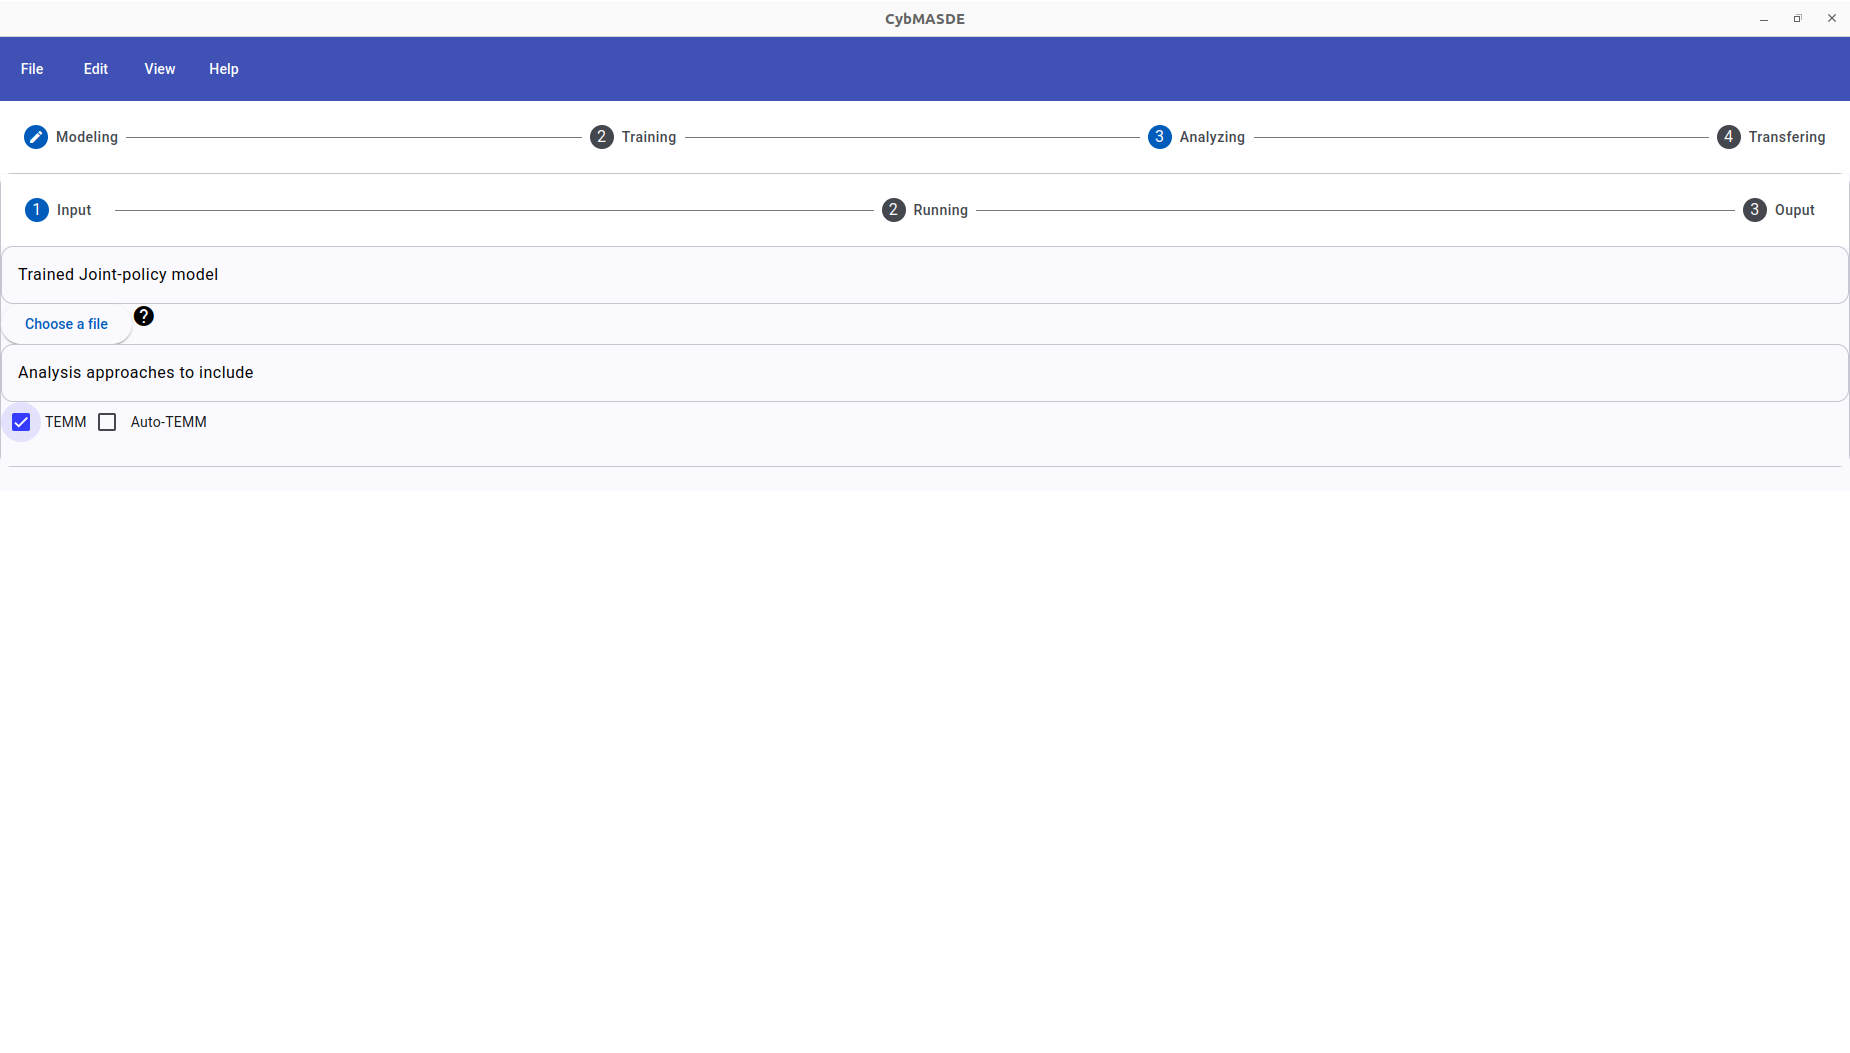
\includegraphics[width=\linewidth]{figures/analyzing_screenshot.png}
       \caption[Capture d'écran de l'onglet analyse de l'interface graphique de CybMASDE]{Capture d'écran de l'interface graphique d'édition du fichier de configuration du projet CybMASDE, illustrant ici l'onglet dédié à l'analyse. Dans cet onglet, l'utilisateur peut configurer les paramètres liés à l'analyse des politiques multi-agents, tels que la méthode à utiliser (\acn{TEMM} ou \acn{Auto-TEMM}) mais aussi les métriques d'évaluation, les visualisations des trajectoires, et les spécifications organisationnelles MOISE+MARL.}
       \label{fig:cybmasde_screenshot_analyzing}
\end{figure}

\begin{figure}[h!]
       \centering
       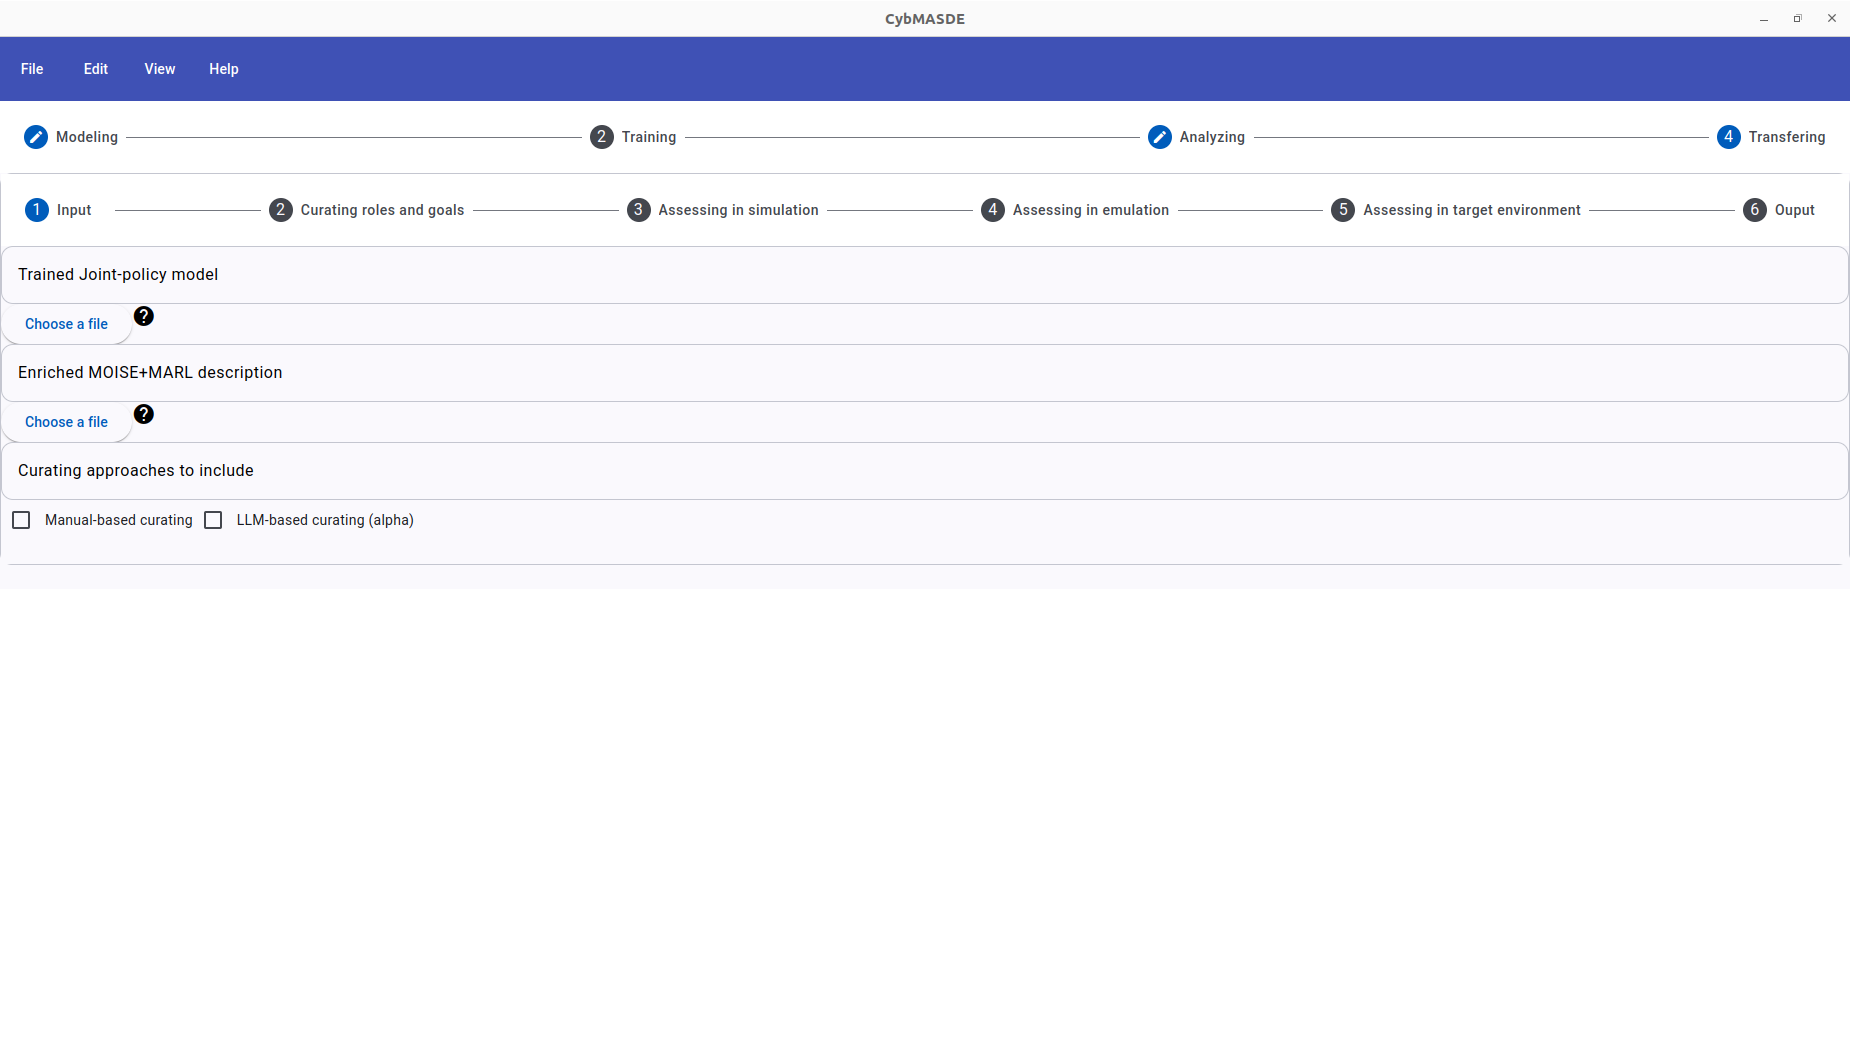
\includegraphics[trim=0cm 15cm 0cm 0cm, clip,width=\linewidth]{figures/refining.png}
       \caption[Capture d'écran de l'onglet raffinement et transfert de l'interface graphique de CybMASDE]{Capture d'écran de l'interface graphique d'édition du fichier de configuration du projet CybMASDE, illustrant ici l'onglet dédié à la phase raffinement et de transfert des politiques. Dans cet onglet, l'utilisateur peut configurer les paramètres liés au raffinement des politiques multi-agents, tels que le nombre maximal d'itérations de raffinement, les critères d'arrêt basés sur la récompense moyenne et la stabilité, ainsi que les options de déploiement des politiques dans l'environnement réel.}
       \label{fig:cybmasde_refining_screenshot}
\end{figure}

\clearpage

\section{API Environnementale de CybMASDE}\label{appendix:cybmasde-environment-api}

Le \autoref{lst:cybmasde_environment_api} présente un extrait du fichier gabarit à utiliser pour implémenter l'API environnementale. Cette API est essentielle pour permettre à \acn{CybMASDE} de communiquer avec l'environnement cible. En implémentant cette interface, l'utilisateur définit les méthodes nécessaires pour récupérer les observations et historiques, appliquer des actions conjointes, et déployer des politiques conjointes dans l'environnement.

\begin{lstlisting}[language=Python,basicstyle=\scriptsize, label={lst:cybmasde_environment_api}, caption={Extrait du fichier gabarit à utiliser pour implémenter l'API environnementale.}]
class EnvironmentAPI:
    """Class representing the environment API for interacting with the environment."""

    def __init__(self):
        pass

    def retrieve_joint_observation(self):
        """Retrieve the joint observation from the environment."""
        # Implement the logic to retrieve the joint observation
        pass

    def retrieve_joint_histories(self):
        """Retrieve the joint histories from the environment."""
        # Implement the logic to retrieve the joint histories
        pass

    def apply_joint_action(self, joint_action):
        """Apply the joint action to the environment."""
        # Implement the logic to apply the joint action
        pass

    def deploy_joint_policy(self, joint_policy):
        """Deploy the joint policy to the environment."""
        # Implement the logic to deploy the joint policy
        pass

\end{lstlisting}

\clearpage

\section{Manuel en ligne de commande de CybMASDE}\label{appendix:cybmasde-manual}

\begin{verbatim}
CYBMASDE(1)                  Manuel de l'utilisateur                  CYBMASDE(1)

NOM
       cybmasde - orchestrer la méthode MAMAD pour la conception de SMA

SYNOPSIS
       cybmasde [commande] [options]

DESCRIPTION
       CybMASDE est une plateforme modulaire permettant de créer, configurer,
       valider, exécuter et analyser des projets de SMA fondés sur le cadre
       MOISE+MARL. Elle supporte l'exécution en ligne de commande (CLI) ou via
       son interface graphique Angular. Le CLI permet une automatisation
       complète (mode batch/HPC) ou une utilisation interactive.

COMMANDES PRINCIPALES
       init        Créer un nouveau projet et générer l'arborescence associée.
       validate    Vérifier la validité du fichier project_configuration.json et des dépendances.
       run         Exécuter un projet complet ou partiel.
       model       Lancer uniquement l'activité de modélisation.
       train       Lancer uniquement l'activité d'entraînement.
       analyze     Lancer uniquement l'activité d'analyse (Auto-TEMM).
       refine      Lancer un cycle de raffinement (analyse + entraînement).
       deploy      Déployer une politique dans l'environnement réel.
       status      Afficher l'état courant du projet (politiques, métriques, logs).
       clean       Nettoyer les fichiers temporaires, traces ou checkpoints inutiles.
       export      Exporter les résultats (politiques, métriques, specs. org.) au format JSON/CSV.
       help        Afficher l'aide générale ou celle d'une commande spécifique.

OPTIONS GÉNÉRALES
       -h, --help
              Afficher l'aide.
       -v, --version
              Afficher la version de CybMASDE.
       -p, --project <path>
              Chemin vers le projet (par défaut: répertoire courant).
       -c, --config <file>
              Spécifier un fichier de configuration alternatif.

SOUS-COMMANDES ET OPTIONS

   init
       cybmasde init -n <nom_projet> [-d <description>] [-o <output_dir>]

       -n, --name <nom>
              Nom du projet.
       -d, --description <texte>
              Description textuelle du projet.
       -o, --output <dir>
              Répertoire de sortie (par défaut: ./<nom_projet>).
       --template <type>
              Type de template d'environnement (handcrafted|worldmodel|minimal).

   validate
       cybmasde validate [-q]

       -q, --quiet
              Ne pas afficher les détails, seulement l'état final (OK/ERREUR).
       --strict
              Considérer tout avertissement comme une erreur.

   run
       cybmasde run [--full-auto | --semi-auto | --manual]

       --full-auto
              Exécuter l'ensemble du pipeline (MTA+T) sans interaction.
       --semi-auto
              Exécution complète mais pause à chaque étape pour confirmation.
       --manual
              Mode manuel : l'utilisateur choisit chaque activité à exécuter.
       --skip-model
              Ne pas relancer la modélisation (utiliser environnement existant).
       --skip-analyze
              Ne pas lancer Auto-TEMM même si la récompense est faible.
       --max-refine <N>
              Nombre maximal d'itérations de raffinement.
       --reward-threshold <val>
              Seuil de récompense moyenne pour arrêt automatique.
       --std-threshold <val>
              Seuil d'écart-type de la récompense pour arrêt du raffinement.
       --accept-inferred
              Accepter automatiquement les spécifications inférées sans validation humaine.
       --interactive-infer
              Afficher les specs inférées et demander validation manuelle (défaut).

   model
       cybmasde model [--auto | --manual] [options]

       --auto
              Utiliser les traces + World Model pour générer l'environnement.
       --manual
              Lancer l'environnement MCAS (handcrafted_environment.py).
       --traces <dir>
              Répertoire contenant des historiques préexistants.
       --vae-dim <val>
              Dimension latente des VAE (défaut: 32).
       --lstm-hidden <val>
              Taille des couches cachées LSTM (64 ou 128).

   train
       cybmasde train [--algo <alg>] [options]

       --algo <nom>
              Algorithme MARL (MAPPO|MADDPG|QMIX|IQL|VDN|ROMA).
       --batch-size <val>
              Taille des batchs (64 ou 128).
       --lr <val>
              Taux d'apprentissage (1e-4 à 5e-4).
       --gamma <val>
              Facteur de discount (0.9 à 0.99).
       --clip <val>
              Valeur de clipping PPO (0.1 à 0.3).
       --seed <val>
              Graine aléatoire.
       --epochs <N>
              Nombre d'époques.

   analyze
       cybmasde analyze [--auto-temm]

       --auto-temm
              Utiliser Auto-TEMM (clustering + optimisation hyperparamètres).
       --metrics <list>
              Sélectionner les métriques d'analyse (reward|stability|org_fit).
       --representativity <val>
              Seuil de représentativité (0.0–1.0).

   refine
       cybmasde refine [--max <N>] [--accept-inferred]

       --max <N>
              Nombre maximum d'itérations de raffinement.
       --accept-inferred
              Accepter automatiquement les specs organisationnelles inférées.
       --interactive
              Demander confirmation utilisateur à chaque cycle (défaut).

   deploy
       cybmasde deploy [--direct | --remote]

       --direct
              Déploiement de la politique sur les agents (mode embarqué).
       --remote
              Politique exécutée par CybMASDE, agents ne reçoivent que les actions.
       --checkpoint <file>
              Spécifier un checkpoint particulier de politique.
       --api <url>
              Spécifier l'URL de l'API environnementale cible.

   status
       cybmasde status

       Affiche l'état du projet : politique active, métriques récentes,
       nombre de cycles MTA, état du transfert.

   clean
       cybmasde clean [--traces | --checkpoints | --all]

       Nettoyer les fichiers temporaires et résultats intermédiaires.

   export
       cybmasde export [--format json|csv|yaml] [--output <dir>]

       Exporter les résultats, politiques et spécifications organisationnelles.

EXEMPLES
       cybmasde init -n infra_test --template worldmodel
       cybmasde validate
       cybmasde run --full-auto --reward-threshold 3.5 --max-refine 5
       cybmasde refine --interactive
       cybmasde deploy --remote --api http://localhost:8080/api

VOIR AUSSI
       Documentation complète : https://github.com/julien6/CybMASDE
       Référence théorique MAMAD et MOISE+MARL dans le manuscrit associé.
\end{verbatim}
